\documentclass{article}
\usepackage{blindtext}
\usepackage[utf8]{inputenc}
\usepackage{amsmath,bm}
\usepackage{amstext}
\usepackage{amsfonts}
\usepackage{amsmath}
\usepackage{multirow}
\usepackage{enumerate}
\usepackage{xeCJK}
\setCJKmainfont{STKaiti}
\usepackage{algorithm}
\usepackage{algorithmic}
\renewcommand{\algorithmicrequire}{ \textbf{输入:}} %Use Input in the format of Algorithm
\renewcommand{\algorithmicensure}{ \textbf{输出:}} %UseOutput in the format of Algorithm
\usepackage{graphicx}
\usepackage{booktabs}
\usepackage{listings}
\lstset{
	columns=fixed,       
	numbers=left,                                        % 在左侧显示行号
	numberstyle=\tiny\color{gray},                       % 设定行号格式
	frame=none,                                          % 不显示背景边框
	keywordstyle=\color[RGB]{40,40,255},                 % 设定关键字颜色
	numberstyle=\footnotesize\color{darkgray},           
	commentstyle=\it\color[RGB]{0,96,96},                % 设置代码注释的格式
	stringstyle=\rmfamily\slshape\color[RGB]{128,0,0},   % 设置字符串格式
	showstringspaces=false,                              % 不显示字符串中的空格
	language=python,                                        % 设置语言
}

\title{Neural Network and Applications\\Homework 2}
\author{陈轶洲 MF20330010}
\begin{document}
	\maketitle
	\numberwithin{equation}{section}
	
\section{回归预测股票价格:利用给定的20天股票数据来预测第21到25天的股票价格}
使用梯度下降法来预测后五天的股票数据,利用python实现单神经元的学习:

\begin{lstlisting}
class singleNN:
	def __init__(self, input_size, lr, iterations, train_data, train_label):
		self.size = input_size
		self.lr = lr
		self.iterations = iterations
	
		self.x_train = train_data
		self.y_label = train_label
		self.y_train = None
	
		self.W = np.random.randn(self.size, 1)
		self.B = np.random.randn(1)
	
		self.loss_list = []
	
	def loss(self):
		self.y_train = self.x_train.dot(self.W) + self.B
		temp = (self.y_train-self.y_label)**2 / 2
		loss = np.sum(temp, axis=0)/temp.shape[0]      
		return loss  
	
	def train(self):
		for i in range(self.iterations):
			self.loss_list.append(self.loss())
			self.y_train = self.x_train.dot(self.W) + self.B
			dy = self.y_train - self.y_label
			dW = self.x_train.T.dot(dy)
			dB = np.sum(dy, axis=0)
			self.W -= self.lr * dW
			self.B -= self.lr * dB
		return self.W, self.B, self.loss_list
	
	def predict(self, x_test):
		y_test = x_test.dot(self.W) + self.B
		return y_test
\end{lstlisting}

将输入神经元的数据规模定义为5,学习率为1e-5,迭代次数为1e5,损失函数为均方误差,初始化模型并进行训练:\\$ 
network = singleNN(input\_size=5, lr=0.000001, iterations=100000, train\_data=x\_data, train\_label=y\_label) $\\

训练过程中记录损失函数:
\begin{figure}[H]
	\centering
	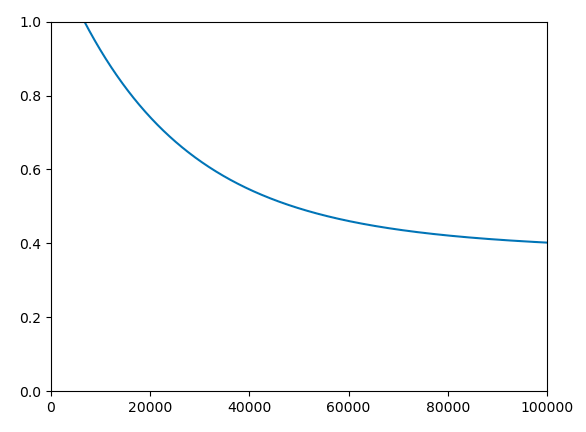
\includegraphics[scale=0.6]{loss.png}
\end{figure}

通过学习得到参数:\\
$ W=[-0.01370438, 0.29370385, -0.0776912, 0.10366604, 0.68671274]^{T} $
$ B=[0.9801407] $\\
\begin{figure}[H]
	\centering
	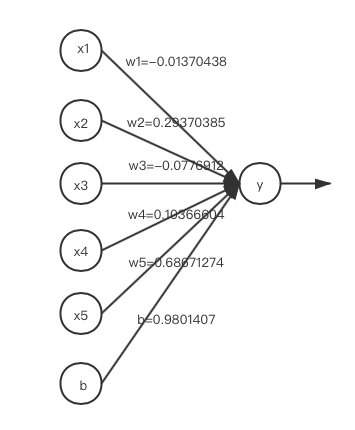
\includegraphics[scale=0.6]{流程图.png}
\end{figure}

利用学习得到的参数对之后天数的股价进行预测:
\begin{table}[htbp]
	\centering
	\caption{第21天到25天预测数据}
	\begin{tabular}{cccccc}
		\toprule    日期 & 21 & 22& 23& 24&25 \\
		\midrule   价格 & 60.96 & 60.57 &  62.14 & 62.39 & 62.40  \\
		\bottomrule   
	\end{tabular}  
\end{table}


\section{"损坏的"LED灯问题}
由题意可知,当$ s=2 $时,状态$x$能正确表达的概率为
\begin{equation}
	p(x|s=2)=\Pi_{j=1}^{7}p(x_j=c_j(2)|s=2)=(1-f)^7
\end{equation}
同理,对于s=3
\begin{equation}
	p(x|s=3)=\Pi_{j=1}^{7}p(x_j=c_j(3)|s=3)=(1-f')^7
\end{equation}
于是,对于给定的$x$,其能正确显示的概率为
\begin{equation}
\begin{aligned}
p(s=2|x) &=\dfrac{p(s=2)p(x|s=2)}{p(x)}\\
&= \dfrac{p(s=2)p(x|s=2)}{p(s=2)p(x|s=2)+p(s=3)p(x|s=3)}\\
&=\dfrac{\frac{1}{2^7}(1-f)^7}{\frac{1}{2^7}(1-f)^7+\frac{1}{2^7}(1-f')^7}\\
&=\dfrac{1}{1+(\frac{1-f'}{1-f})^7}
\end{aligned}
\end{equation}
同理可得
\begin{equation}
	\begin{aligned}
		p(s=3|x) = \dfrac{1}{1+(\frac{1-f}{1-f’})^7}
	\end{aligned}
\end{equation}
综上,显示数字2或3的概率为
\begin{equation}
p(s=2\cup s=3|x)=\dfrac{1}{1+(\frac{1-f}{1-f'})^7}+\dfrac{1}{1+(\frac{1-f'}{1-f})^7}
\end{equation}
\end{document}
